\documentclass[oneside,12pt]{classes/thesis}

% PDF Meta-data
\ifpdf
    \pdfinfo {
		/Title  (Bsc Thesis)
        /Creator (TeX)
        /Producer (pdfTeX)
        /Author (Papadopoulos Nikos nikpapas@gmail.com)
        /CreationDate (D:20110101000000)  %format D:YYYYMMDDhhmmss
        /ModDate (D:2011815213532)
        /Subject (Ray tracing, Theory and implementation)
        /Keywords (Bsc, Thesis, Ray tracing)
	}
    \pdfcatalog 
	{ 
		/PageMode (/UseOutlines)
        /OpenAction (fitbh)  
	}
\fi

% Cover
% - Title
\title
{
		Ray tracing\\[1ex]
        Θεωρία και υλοποίηση
}

\supervisor{Επιβλέπων καθηγητής}
\supervprof{Θέμης Παναγιωτόπουλος}

% - Body
\ifpdf
	\author{\href{mailto:nikpapas@gmail.com}{Παπαδόπουλος Νικόλαος}}
	\collegeordept{\href{http://www.cs.unipi.gr}{Τμήμα πληροφορικής}}
	\university{\href{http://www.unipi.gr}{Πανεπιστήμιο Πειραιώς}}
	% crest logo
	\crest{
\includegraphics[width=30mm]{unipi}}
\else
	\author{Παπαδόπουλος Νικόλαος}
	\collegeordept{Τμήμα πληροφορικής}
	\university{Πανεπιστήμιο Πειραιώς}
	\crest{
\includegraphics[bb = 0 0 292 336, width=30mm]{unipi}}
\fi

\renewcommand{\submittedtext}{Πτυχιακή εργασία}
%\degree{}
\degreedate{2011}

% turn of those nasty overfull and underfull hboxes
\hbadness=10000
\hfuzz=50pt

% Comment out the next line to get single spacing
%\onehalfspacing

\begin{document}

\maketitle

%set the number of sectioning levels that get number and appear in the contents
\setcounter{secnumdepth}{3}
\setcounter{tocdepth}{3}

\frontmatter % book mode only
\pagenumbering{roman}
%% Thesis Dedication ---------------------------------------------------

\begin{dedication}

\end{dedication}

% ----------------------------------------------------------------------

%% Thesis Acknowledgements ------------------------------------------------

%\begin{acknowledgementslong} %uncommenting this line, gives a different acknowledgements heading
\begin{acknowledgements}      %this creates the heading for the acknowlegments

\end{acknowledgements}
%\end{acknowledgmentslong}

% ------------------------------------------------------------------------

% Thesis Abstract -----------------------------------------------------

\chapter{Περίληψη}

\paragraph{} % the abstract

\begin{sloppypar}
Η τεχνική του raytracing χρησιμοποιείται για την δημιουργία συνθετικών εικόνων ακολουθώντας
τη πορεία του φωτός καθώς αυτό περνάει απο το κάθε εικονοστοιχείο του επιπέδου προβολής.
Με αυτό το τρόπο μπορούμε με ευκολία να δημιουργήσουμε φωτορεαλιστικές απεικονίσεις ενός
μαθηματικά μοντελοποιημένου περιβάλλοντος, κάτι στο οποίο άλλες τεχνικές υστερούν. Η 
παρούσα μελέτη έχει ως σκοπό την παρουσίαση των βασικών αλγορίθμων πίσω από τη τεχνική του 
ray tracing, καθώς και τη διερεύνηση πιθανών υπολογιστικών βελτίστοποιήσεων με σκοπό την 
ελαχιστοποίηση του χρόνου και των πόρων που απαιτούνται για την σύνθεση της τελικής εικόνας.
Επιπλέον παρουσιάζεται το μαθηματικό πλαίσιο που ορίζει τις ιδιότητες των οντοτήτων και τα 
φυσικά μοντέλα τα οποία χρησιμοποιεί η εν λόγω τεχνική. Τέλος γίνεται υλοποίηση των 
παρουσιαζόμενων τεχνικών και αλγορίθμων.
\end{sloppypar}

% ----------------------------------------------------------------------


% Contents
\renewcommand{\contentsname}{Περιεχόμενα}
\tableofcontents

% Figures
\renewcommand*\listfigurename{Λίστα εικόνων}
\listoffigures

% Chapters
\renewcommand{\chaptername}{Kεφάλαιο}
\mainmatter % book mode only
% Thesis Introduction 
\chapter{Εισαγωγή}

\ifpdf
    \graphicspath{{Introduction/IntroductionFigs/PNG/}{Introduction/IntroductionFigs/PDF/}{Introduction/IntroductionFigs/}}
\else
    \graphicspath{{Introduction/IntroductionFigs/EPS/}{Introduction/IntroductionFigs/}}
\fi

\begin{sloppypar}

\paragraph{}
Για να αναπαραστήσουμε ένα εικονικό περιβάλλον σε ένα υπολογιστικό σύστημα,
είναι απαραίτητο να βρεθεί μια μαθηματική περιγραφή των οντοτήτων που εμπεριέχονται σε αυτό, 
των ιδιοτήτων τους, καθώς και του τρόπου με τον οποίο αυτές αλληλεπιδρούν μεταξύ τους. 
Για το σκοπό αυτό έχουν αναπτυχθεί διάφορες τεχνικές, καθε μια από τις οποίες έχει διαφορετικές 
εφαρμογές ανάλογα με τα χαρακτηριστικά της. Η πιο διαδεδομένη από αυτές τις τεχνικές στη σφαίρα 
των real time απεικονίσεων, είναι αυτή του scanline rendering. Αυτό οφείλεται στο ότι μπορεί 
να δημιουργήσει αρκετά πειστικές εικόνες γρήγορα. Εν τούτοις υπάρχουν περιορισμοί στην οπτική 
πιστότητα του αποτελέσματος, κυρίως διότι δεν μοντελοποιούνται οι φυσικές ιδιότητες του πραγματικού 
κόσμου αλλά χρησιμοποιούνται αφαιρετικά προσεγγιστικά μοντέλα. Αυτό το κενό έρχεται να καλύψει 
εν μέρει η τεχνική του ray tracing.

\paragraph{}
Με τον όρο ray tracing αναφερόμαστε στην τεχνική η οποία χρησιμοποιείται για τη δημιουργία μίας
εικόνα, ακολουθώντας την πορεία του φωτός καθώς αυτό περνάει μέσα από τα διακριτά εικονοστοιχεία 
του επιπέδου προβολής και κινείται μεσα σε μια σκηνή, αλλάζοντας πορεία επηρεαζόμενο από τις 
ιδιότητες που χαρακτηρίζουν κάθε επιφάνεια στην οποία αυτό προσπίπτει. Έτσι μπορούμε να έχουμε 
αντικείμενα με ημιδιαφανείς επιφάνειες, με διαφορετικές υφές και χρώματα, οι οποίες προκαλούν 
την ανάκλαση ή την διάθλαση του φωτός αλλαζοντας τη πορεία του. Για παράδειγμα, αν έχουμε τέσσερεις 
κρυστάλλινες σφαίρες, διαφορετικού χρώματος και μεγέθους, τη μία πολύ κοντά στην άλλη, θα πρέπει 
στην επιφάνεια της κάθε μπάλας να αποτυπώνονται οι υπόλοιπες τέσσερις, όχι μόνο το είδωλο τους, 
αλλά τόσο το χρώμα, όσο και το μέγεθός τους όπως θα γινόταν και σε ένα πραγματικό περιβάλλον. 
Παρακάτω θα παρουσιαστούν οι τεχνικές που χρησιμοποιούνται για να επιτύχουμε αυτό το αποτέλεσμα 
καθως και το πλήρες μαθηματικό υπόβαθρο πίσω από αυτές.

\end{sloppypar}

\chapter{Ο βασικός αλγόριθμος.}

\ifpdf
    \graphicspath{{Chapter1/Chapter1Figs/PNG/}{Chapter1/Chapter1Figs/PDF/}{Chapter1/Chapter1Figs/}}
\else
    \graphicspath{{Chapter1/Chapter1Figs/EPS/}{Chapter1/Chapter1Figs/}}
\fi

\section{Γενικά για τη μέθοδο}

\begin{sloppypar}

\paragraph{}
	Το ray tracing είναι μια τεχνική που χρησιμοποιείται στο πεδίο των γραφικών για τη
δημιουργία συνθετικών απεικονίσεων ένος μαθηματικά μοντελοποιημένου περιβάλλοντος. Η μέθοδος
αυτή προσπαθεί να εξομοιώσει τις ιδιότητες του φωτός και την συμπεριφορά του καθώς αυτό προσπίπτει
στις διάφορες επιφάνειες ενός χώρου. Είναι εύκολο κανείς να αντιληφθεί ότι μια τέτοια εξομοίωση θα
απαιτούσε τον αυστηρό ορισμό όλων των φυσικών ιδιοτήτων του φωτός και των οντοτήτων που αλληλεπιδρούν
με αυτό καθώς και μεγάλη υπολογιστική δύναμη. Κάτι τέτοιο αν και θα οδηγούσε σε απεικονίσεις που 
χαρακτηρίζονται απο εξαιρετικά υψηλό βαθμό ρεαλισμού, εν τούτοις παρουσιάζει μεγάλες δυσκολίες που 
καθιστούν την μέθοδο πρακτικά μη υλοποιήσιμη και τουλάχιστον με την παρούσα τεχνολογία, 
υπολογιστικά αδύνατη.

\paragraph{}
	Το ερώτημα λοιπόν που προκύπτει αμέσως είναι, με ποιον τρόπο μπορούμε να απλοποιήσουμε το φυσικό
μοντέλο που περιγράφει της αλληλεπιδράσεις αυτές ώστε να κάνουμε μια τέτοια εξομοίωση υπολογιστικά 
εφικτή. Η απάντηση είναι απλή. Λειτουργούμε αφαιρετικά με σκοπό την προσέγγιση ενός ρεαλιστικού
αποτελέσματος. Όπως θα δούμε και στη συνέχεια, στην μέθοδο του ray tracing κάνουμε αρκετές παραδοχές 
με σκοπό να ελαχιστοποιηθεί το υπολογιστικό κόστος.

\end{sloppypar}
 
	

Here is an equation\footnote{the notation is explained in the nomenclature section :-)}:
\begin{eqnarray}
CIF: \hspace*{5mm}F_0^j(a) &=& \frac{1}{2\pi \iota} \oint_{\gamma} \frac{F_0^j(z)}{z - a} dz
\end{eqnarray}

\section{Σκίαση}
and here I write more ...\cite{texbook}

\subsection{Aνακλάσεις}
... and some more ...

Now I would like to cite the following: \cite{latex} and \cite{texbook}
%and \cite{Rud73}.

I would also like to include a picture ...

\begin{figure}[!htbp]
  \begin{center}
    \leavevmode
    \ifpdf
%      \includegraphics[height=6in]{aflow}
    \else
 %     \includegraphics[bb = 92 86 545 742, height=6in]{aflow}
    \fi
    \caption{Airfoil Picture}
    \label{FigAir}
  \end{center}
\end{figure}

% above code has been macro-fied in Classes/MacroFile.tex file
%\InsertFig{\IncludeGraphicsH{aflow}{6in}{92 86 545 742}}{Airfoil Picture}{FigAir}

So as we have now labelled it we can reference it, like so (\ref{FigAir}) and it
is on Page \pageref{FigAir}. And as we can see, it is a very nice picture and we
can talk about it all we want and when we are tired we can move on to the next
chapter ...

I would also like to add an extra bookmark in acroread like so ...
\ifpdf
  \pdfbookmark[2]{bookmark text is here}{And this is what I want bookmarked}
\fi
% ------------------------------------------------------------------------


%%% Local Variables: 
%%% mode: latex
%%% TeX-master: "../thesis"
%%% End: 

\chapter{Σκίαση}

\begin{sloppypar}

\section{Μοντέλα σκίασης}

\subsection{Lambert}

\subsection{Phong}

\subsection{Blinn-Phong}

\section{Εφέ}

\subsection{Ανάκλαση}

\subsection{Διάθλαση}

\end{sloppypar}

% ------------------------------------------------------------------------

\chapter{Θεμελιώδη γεωμετρικά σχήματα}

\begin{sloppypar}

\section{Σφαίρα}
\paragraph{}

\section{Επίπεδο}
\paragraph{}

\section{Τρίγωνο}
\paragraph{}

\end{sloppypar}

% ------------------------------------------------------------------------

% Conclusions ----------------------------------------------------------

\def\baselinestretch{1}

\chapter{Συμπεράσματα}

\ifpdf
    \graphicspath{{Conclusions/ConclusionsFigs/PNG/}{Conclusions/ConclusionsFigs/PDF/}{Conclusions/ConclusionsFigs/}}
\else
    \graphicspath{{Conclusions/ConclusionsFigs/EPS/}{Conclusions/ConclusionsFigs/}}
\fi

\def\baselinestretch{1.66}

Έχοντας δει τους βασικούς αλγόριθμους της τεχνικής του ray tracing μπορούμε να καταλήξουμε σε
κάποια συμπεράσματα.

% ----------------------------------------------------------------------


% Appendices
\backmatter % book mode only
\appendix
\chapter{Παράρτημα Α - Δείγματα εικόνων}

\DeclareGraphicsExtensions{.pdf,.png,.jpg}
\graphicspath{{appendix1/fig/}}

\begin{figure} 
\centering 
%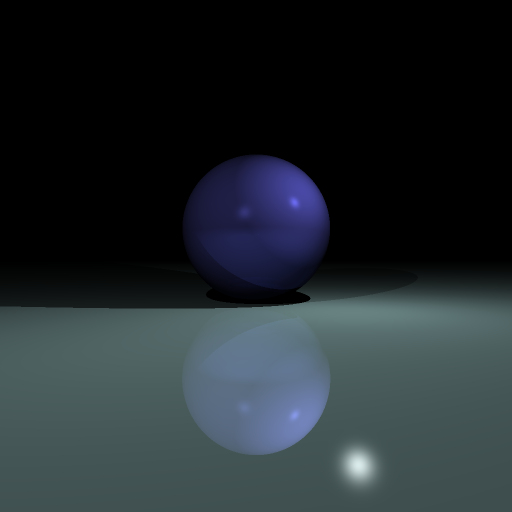
\includegraphics[width=90mm, height=90mm, keepaspectratio=true]{scn_sphere}
\caption{H σκηνή sphere}
\end{figure}

\begin{figure} 
\centering 
%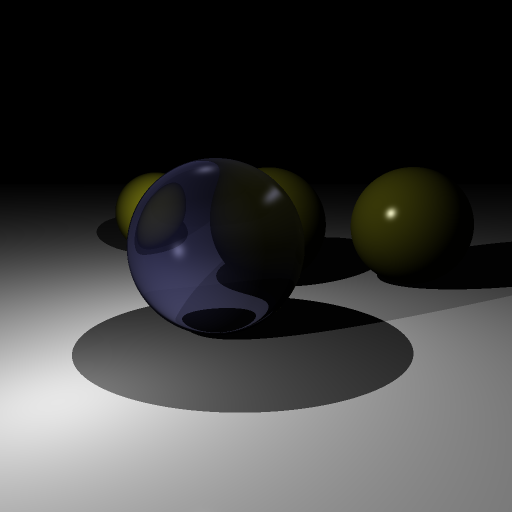
\includegraphics[width=90mm, height=90mm, keepaspectratio=true]{scn_refraction}
\caption{H σκηνή refraction}
\end{figure}

\begin{figure} 
\centering 
%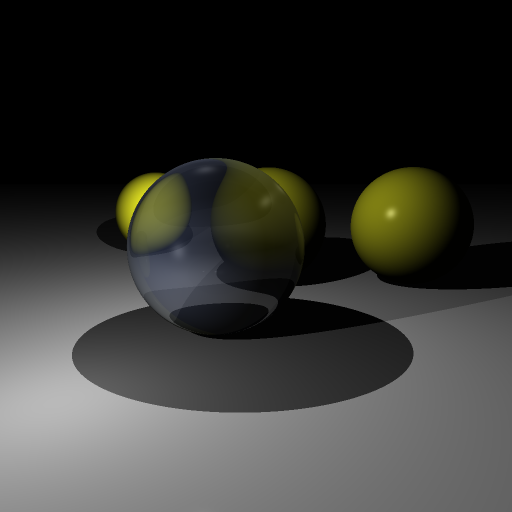
\includegraphics[width=90mm, height=90mm, keepaspectratio=true]{scn_refraction_1033}
\caption{H σκηνή refraction με διαφορετικό material}
\end{figure}

\begin{figure} 
\centering 
%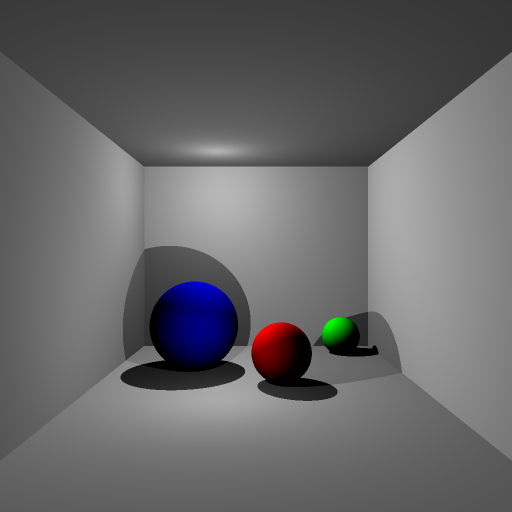
\includegraphics[width=90mm, height=90mm, keepaspectratio=true]{scn_room_lambert}
\caption{H σκηνή room lambert}
\end{figure}

\begin{figure} 
\centering 
%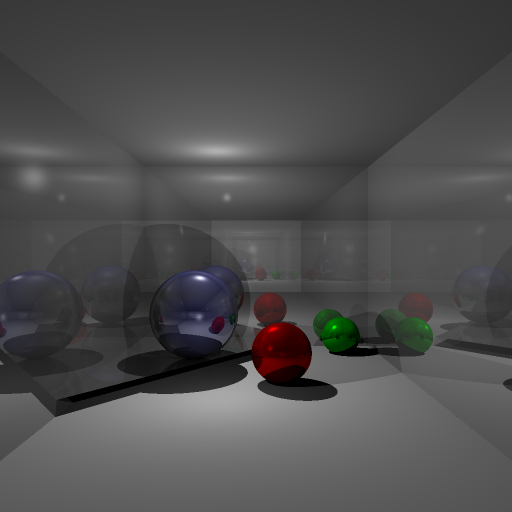
\includegraphics[width=90mm, height=90mm, keepaspectratio=true]{scn_room_phong}
\caption{H σκηνή room phong}
\end{figure}

\begin{figure} 
\centering 
%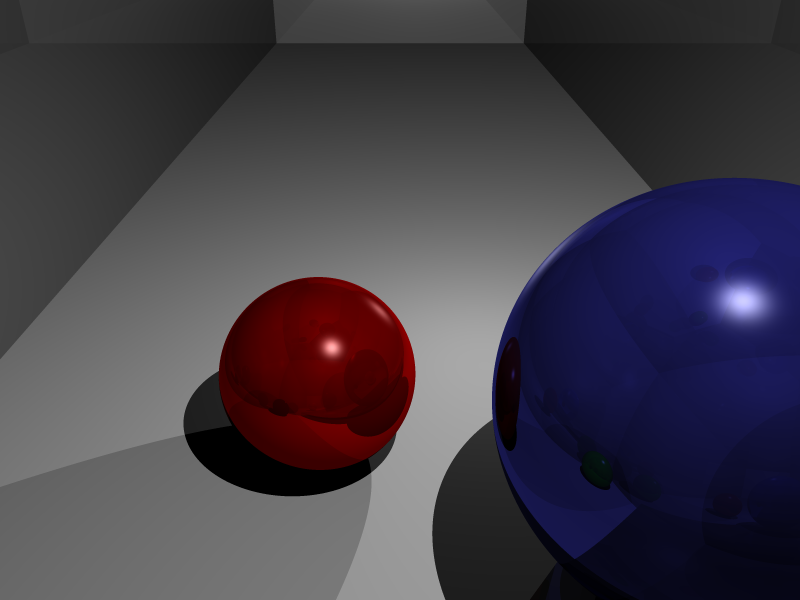
\includegraphics[width=90mm, keepaspectratio=true]{scn_room_2}
\caption{H σκηνή room phong από άλλη κάμερα}
\end{figure}

\begin{figure} 
\centering 
%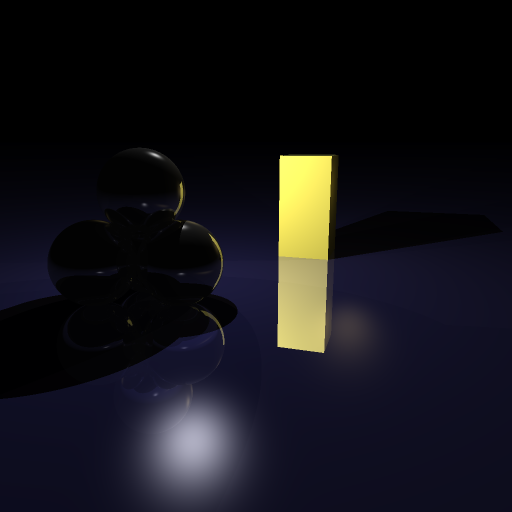
\includegraphics[width=90mm, height=90mm, keepaspectratio=true]{scn_trophy}
\caption{H σκηνή trophy}
\end{figure}

\begin{figure} 
\centering 
%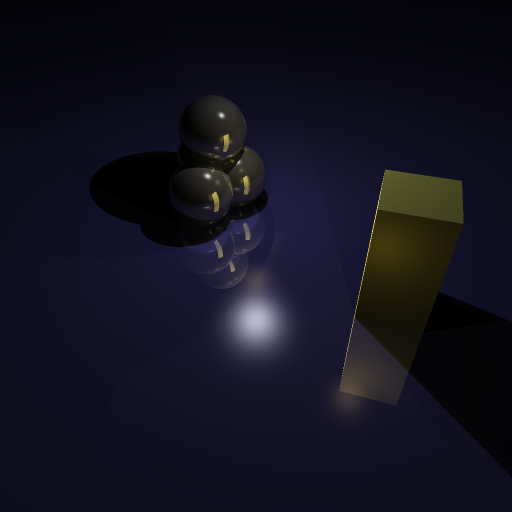
\includegraphics[width=90mm, height=90mm, keepaspectratio=true]{scn_trophy_2}
\caption{H σκηνή trophy από άλλη κάμερα}
\end{figure}

\begin{figure} 
\centering 
%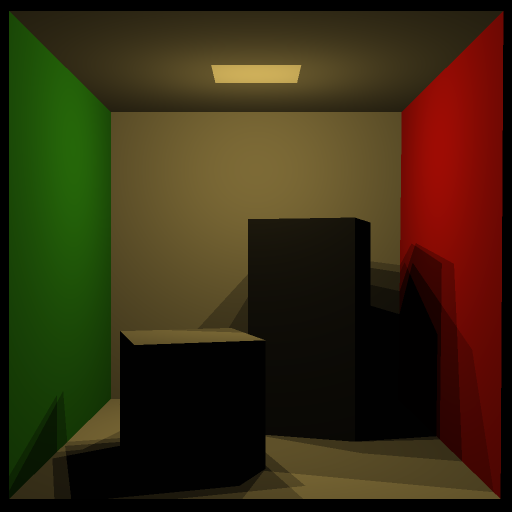
\includegraphics[width=90mm, height=90mm, keepaspectratio=true]{scn_cornell_box}
\caption{H σκηνή cornell box}
\end{figure}

\begin{figure} 
\centering 
%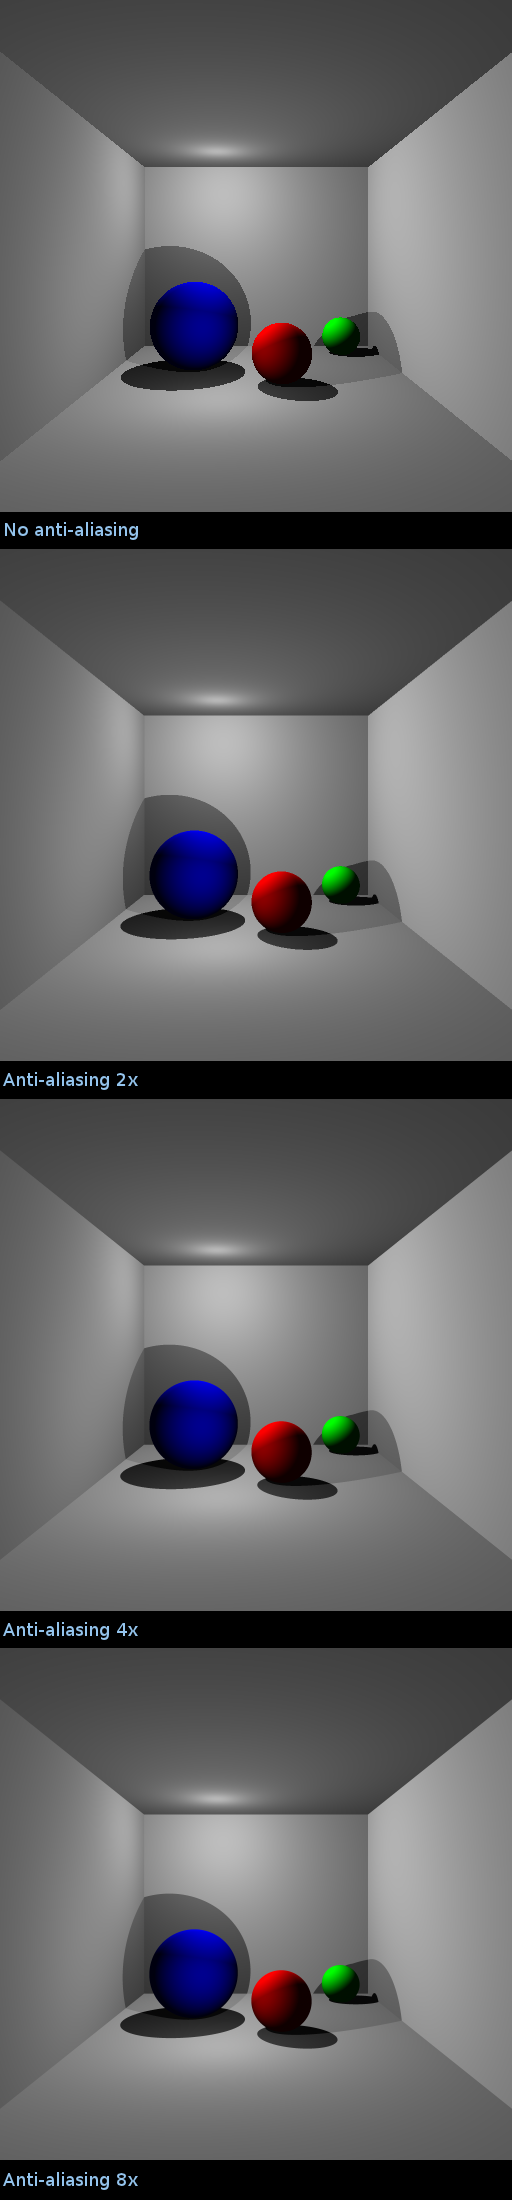
\includegraphics[width=40mm, keepaspectratio=true]{scn_antialiasing}
\caption{Antialiasing}
\end{figure}

\begin{figure} 
\centering 
%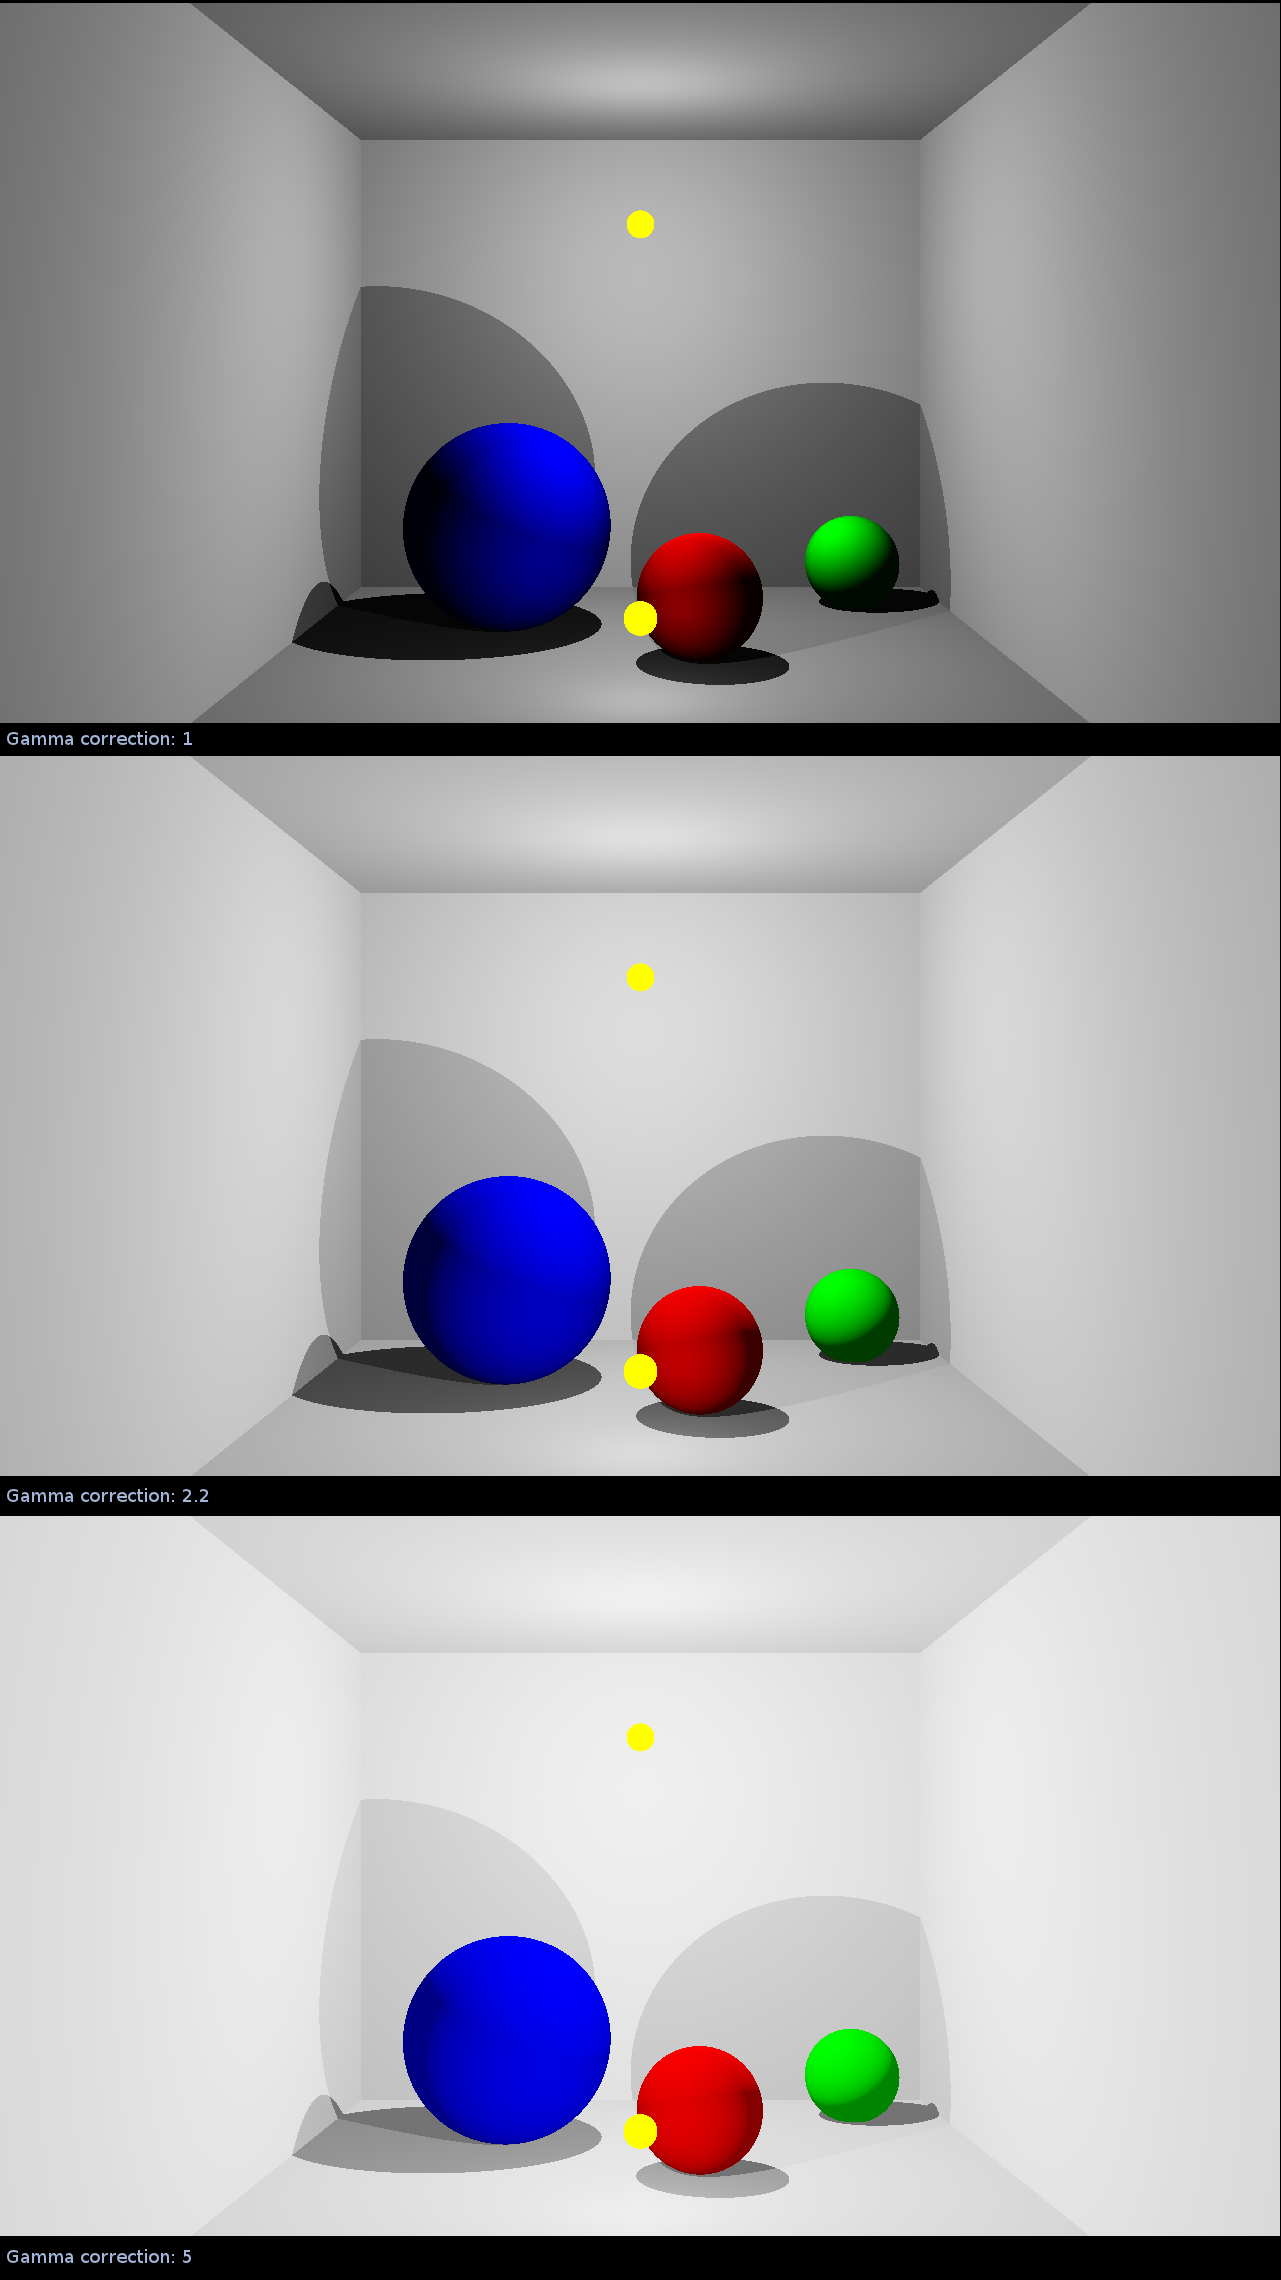
\includegraphics[width=70mm, keepaspectratio=true]{scn_gamma}
\caption{Gamma correction}
\end{figure}

\chapter{Παράρτημα Β - Κώδικας}

% ------------------------------------------------------------------------


% Bibliography
\bibliographystyle{classes/biblio}
\renewcommand{\bibname}{Βιβλιογραφικές πηγές} % changes default name Bibliography to References
\bibliography{references/references} % References file

\end{document}
